% methodologie/AnalyseExploratoireDesDonnees.tex

\subsection{Analyse Exploratoire Des Donnees}
\subsubsection{La distribution des scores}
\begin{figure}[h]
    \centering
    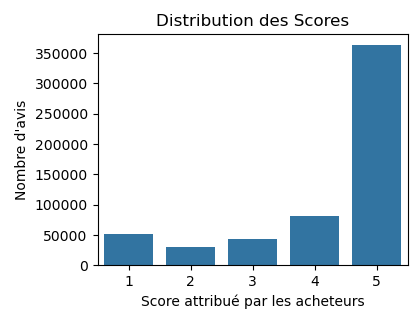
\includegraphics[scale=0.8]{assets/distrubutiondesscores.PNG}
    \caption{La distrubution des scores}
    \label{fig:distrubution_des_scores}
\end{figure}

Analysons les résultats du graphique :

\begin{itemize}
    \item Score 5 : Il y a 363,122 occurrences où le score est égal à 5.
    \item Score 4 : Il y a 80,655 occurrences où le score est égal à 4.
    \item Score 1 : Il y a 52,268 occurrences où le score est égal à 1.
    \item Score 3 : Il y a 42,640 occurrences où le score est égal à 3.
    \item Score 2 : Il y a 29,769 occurrences où le score est égal à 2.
\end{itemize}

Ces résultats offrent une vision détaillée de la distribution des scores dans l'ensemble de données. Notamment, le score 5 est nettement plus fréquent que les autres, suggérant une prédominance d'évaluations positives. À l'inverse, les scores 1, 2 et 3 sont moins fréquents, indiquant une proportion moindre d'évaluations négatives ou neutres. Cette information est précieuse pour appréhender la tendance globale des évaluations dans l'ensemble de données.

\subsubsection{Calcul de la moyenne et de la médiane des scores dans les données}


Le calcul de la moyenne et de la médiane des scores dans les données donne les résultats suivants :

\[
\text{Moyenne des scores : } 4.18
\]
\[
\text{Médiane des scores : } 5.0
\]

Comme observé, la majorité des scores se situent entre 4 et 5, avec une moyenne de 4.18. En raison de la distribution très inclinée vers la gauche, nous envisageons une prédiction binaire. Les avis avec un score entre 1 et 3 seront considérés comme négatifs, tandis que ceux avec un score de 4 ou 5 seront considérés comme positifs. Cette approche simplifiée prend en compte la tendance vers des évaluations positives dans l'ensemble de données.


\subsubsection{Distribution des Sentiments}
\begin{figure}[h]
    \centering
    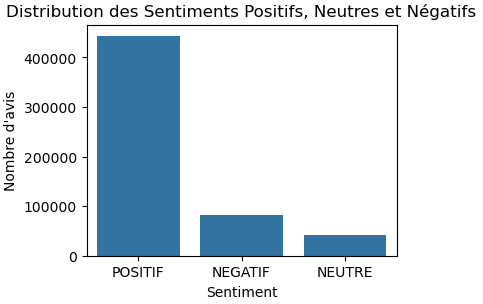
\includegraphics[scale=0.8]{assets/distrubutiondessentiments.PNG}
    \caption{Distribution des Sentiments Positifs, Neutres et Négatifs}
    \label{fig:distrubution_des_sentiments}
\end{figure}

Les résultats du graphique montrent que le nombre d'avis positifs ("POSITIF") est le plus élevé, totalisant 443,756 occurrences. Les avis négatifs ("NEGATIF") s'élèvent à 82,007, tandis que les avis neutres ("NEUTRE") sont au nombre de 42,638. Cette répartition permet une visualisation claire de la distribution des sentiments dans l'ensemble de données.